\titre{}
\theme{calcDiff}
\auteur{Nathan Scheinmann}
\niveau{3M}
\source{}
\type{serie}
\piments{1}
\pts{}
\annee{2526}

\contenu{
	\tcblower
Un rectangle est inscrit entre l'axe des $x$ et l'arc de parabole d'équation $y=4-x^2$ (voir l'illustration) Trouvez les dimensions du rectangle d'aire maximale.
\begin{center}
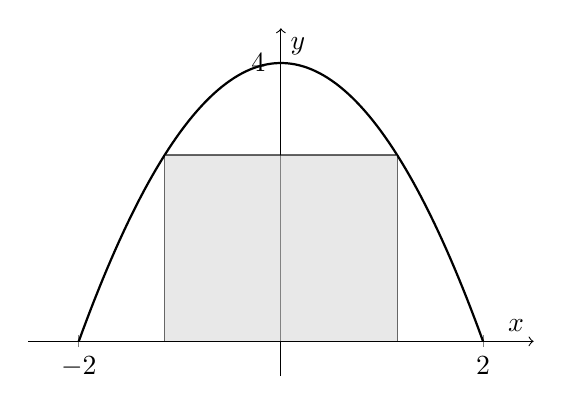
\begin{tikzpicture}
    \begin{axis}[
        axis lines = middle,
        xlabel = {$x$},
        ylabel = {$y$},
        xmin = -2.5, xmax = 2.5,
        ymin = -0.5, ymax = 4.5,
        xtick = {-2, 2},
        ytick = {4},
        width=8cm,
        height=6cm,
        axis line style={->},
    ]
        % Draw the parabola y = 4 - x^2
        \addplot [
            domain=-2:2,
            samples=100,
            thick,
            black
        ] {4 - x^2};

        % Draw an example inscribed rectangle
        % Let's pick x = 1.15 (approximate for visualization)
        \draw[fill=gray!30, opacity=0.6] (axis cs:-1.15, 0) rectangle (axis cs:1.15, 2.6775);
    \end{axis}
\end{tikzpicture}
\end{center}
}
\correction{
	\tcblower

}
